\documentclass[10pt]{article}
\usepackage[margin=0.4in]{geometry}
\usepackage{amsmath}
\usepackage{enumitem}
\usepackage{multicol}
\usepackage{tikz}
\usetikzlibrary{shapes.geometric}
\usepackage{soul}

\newcommand{\ds}{\displaystyle}
\newcommand{\on}{\operatorname}


\begin{document}
\newcounter{enumCount}
\pagestyle{empty}
\subsection*{Homework 2 - Math 243 \hfill Name: \underline{\hspace*{2in}}}

\noindent

\begin{enumerate}
\item Suppose that a simple electric circuit has a resistor with resistance $R$ in ohms ($\Omega$), a capacitor with capacitance $C$ in farads (F) and a (time-dependent) voltage source that provides $E(t)$ volts (V).  The voltage drop across the capacitor $E_C$ satisfies the differential equation
$$RC \dfrac{dE_C}{dt} + E_C = E(t).$$
Solve this differential equation if $E(t)$ is a constant $5$ volts, and $R = 2~\Omega$ and $C = 1$ F with initial condition $E_C(0) = 10$ V. 
\vfill

\item Draw a rough sketch of a slope field for the following differential equations. 
\begin{center}
\begin{tikzpicture}[scale=0.8]
\draw (-3.5, 4) node[right] {(a) $y' = -xy$};
\draw[gray!40] (-2.5,-2.5) grid (2.5, 2.5);
\draw[thick,<->] (-3,0) -- (3,0);
\draw[thick,<->] (0,-3) -- (0,3);

\begin{scope}[xshift =12cm]
\draw (-3.5, 4) node[right] {(b) $y' = (x+1)(x-2)$};
\draw[gray!40] (-2.5,-2.5) grid (2.5, 2.5);
\draw[thick,<->] (-3,0) -- (3,0);
\draw[thick,<->] (0,-3) -- (0,3);
\end{scope}
\end{tikzpicture}
\end{center}
\bigskip

\item Match each of the following differential equations to one of the slope fields below: $y' = 1-x$, $y'=x-2y$, and $y' = x(1-y)$.  Justify your answer. 
\begin{center}
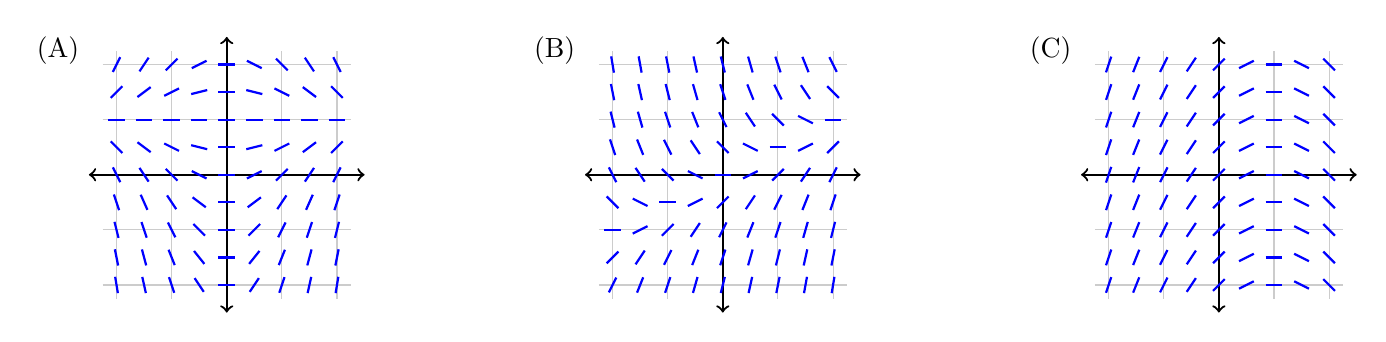
\begin{tikzpicture}[scale=0.7]
\begin{scope}
\draw (-2.5,2.25) node[left] {(A)};
\def\xmax{2}; 
\def\xmin{-2};
\def\xstep{0.5};
\def\ymax{2};
\def\ymin{-2};
\def\ystep{0.5};
\def\ext{0.5};  % how far axes extend past last tick mark
\def\w{0.15};    % radius of the scaled slope vector
\pgfmathparse{\xmin+\xstep};
\let\xnext\pgfmathresult;
\pgfmathparse{\ymin+\ystep};
\let\ynext\pgfmathresult;
\draw[gray!40] (\xmin-\ext/2,\ymin-\ext/2) grid (\xmax+\ext/2,\ymax+\ext/2);
\draw[thick,<->] (\xmin-\ext,0) -- (\xmax+\ext,0);
\draw[thick,<->] (0,\ymin-\ext) -- (0,\ymax+\ext);
\foreach \x in {\xmin,\xnext,...,\xmax} { 
	\foreach \y in {\ymin,\ynext,...,\ymax} {
		\pgfmathparse{\x*(1-\y)}; 	% Enter your differential equation here.  
		\let\m\pgfmathresult;  % \m is the slope
		\pgfmathparse{sqrt(1+\m*\m)};
		\let\n\pgfmathresult;  % \n is the radius of the unscaled slope vector
		\pgfmathparse{\w/\n};	
		\let\dx\pgfmathresult;   
		\pgfmathparse{\dx*\m};	
		\let\dy\pgfmathresult;
		\draw[thick,color=blue] (\x-\dx,\y-\dy) -- (\x+\dx,\y +\dy);
	}
}
\end{scope}


\begin{scope}[xshift=9cm]
\draw (-2.5,2.25) node[left] {(B)};
\def\xmax{2}; 
\def\xmin{-2};
\def\xstep{0.5};
\def\ymax{2};
\def\ymin{-2};
\def\ystep{0.5};
\def\ext{0.5};  % how far axes extend past last tick mark
\def\w{0.15};    % radius of the scaled slope vector
\pgfmathparse{\xmin+\xstep};
\let\xnext\pgfmathresult;
\pgfmathparse{\ymin+\ystep};
\let\ynext\pgfmathresult;
\draw[gray!40] (\xmin-\ext/2,\ymin-\ext/2) grid (\xmax+\ext/2,\ymax+\ext/2);
\draw[thick,<->] (\xmin-\ext,0) -- (\xmax+\ext,0);
\draw[thick,<->] (0,\ymin-\ext) -- (0,\ymax+\ext);
\foreach \x in {\xmin,\xnext,...,\xmax} { 
	\foreach \y in {\ymin,\ynext,...,\ymax} {
		\pgfmathparse{(\x-2*\y)}; 	% Enter your differential equation here.  
		\let\m\pgfmathresult;  % \m is the slope
		\pgfmathparse{sqrt(1+\m*\m)};
		\let\n\pgfmathresult;  % \n is the radius of the unscaled slope vector
		\pgfmathparse{\w/\n};	
		\let\dx\pgfmathresult;   
		\pgfmathparse{\dx*\m};	
		\let\dy\pgfmathresult;
		\draw[thick,color=blue] (\x-\dx,\y-\dy) -- (\x+\dx,\y +\dy);
	}
}
\end{scope}

\begin{scope}[xshift=18cm]
\draw (-2.5,2.25) node[left] {(C)};
\def\xmax{2}; 
\def\xmin{-2};
\def\xstep{0.5};
\def\ymax{2};
\def\ymin{-2};
\def\ystep{0.5};
\def\ext{0.5};  % how far axes extend past last tick mark
\def\w{0.15};    % radius of the scaled slope vector
\pgfmathparse{\xmin+\xstep};
\let\xnext\pgfmathresult;
\pgfmathparse{\ymin+\ystep};
\let\ynext\pgfmathresult;
\draw[gray!40] (\xmin-\ext/2,\ymin-\ext/2) grid (\xmax+\ext/2,\ymax+\ext/2);
\draw[thick,<->] (\xmin-\ext,0) -- (\xmax+\ext,0);
\draw[thick,<->] (0,\ymin-\ext) -- (0,\ymax+\ext);
\foreach \x in {\xmin,\xnext,...,\xmax} { 
	\foreach \y in {\ymin,\ynext,...,\ymax} {
		\pgfmathparse{(1-\x)}; 	% Enter your differential equation here.  
		\let\m\pgfmathresult;  % \m is the slope
		\pgfmathparse{sqrt(1+\m*\m)};
		\let\n\pgfmathresult;  % \n is the radius of the unscaled slope vector
		\pgfmathparse{\w/\n};	
		\let\dx\pgfmathresult;   
		\pgfmathparse{\dx*\m};	
		\let\dy\pgfmathresult;
		\draw[thick,color=blue] (\x-\dx,\y-\dy) -- (\x+\dx,\y +\dy);
	}
}
\end{scope}
\end{tikzpicture}
\end{center}
\bigskip

%\item Recall that $\dfrac{dy}{dt} = - \alpha y$ is the equation for exponential decay.  It can be used to model things like radioactive decay and population decline, among other things.  Consider the following variation of this equation (assume that both $\alpha, \beta >0$):
%$$\dfrac{dy}{dt} = - \alpha y + \beta.$$
%Describe in words one thing that this equation might be useful to model.
%\vfill

\item Seawater has about 3.5 grams of salt per liter.  Suppose that a pool is filled with 10{,}000 liters of seawater.  If 200 liters of fresh water evaporate from the pool every hour, and 200 liters of seawater are added to the pool to keep the volume of water in the pool constant, then find a differential equation to model the amount of salt in the pool as a function of time.  You do not need to solve the differential equation.  
\vfill

\newpage



\setcounter{enumCount}{\theenumi}
\end{enumerate}

\noindent
\textit{For each of the following autonomous differential equations, find all equilibrium values of $y$. For each one, say whether it is a stable or unstable equilibrium.}

\begin{multicols}{3}
\begin{enumerate}
\setcounter{enumi}{\theenumCount}
\item $\dfrac{dy}{dt} = 2y - 3$


\item $\dfrac{dy}{dt} = y^2 - 6y + 5$.

\item $\dfrac{dy}{dt} = 2 \sin y$. 

\setcounter{enumCount}{\theenumi}
\end{enumerate} 
\end{multicols}

\vfill

\begin{enumerate}
\setcounter{enumi}{\theenumCount}
\item Suppose that the population of fish in a lake satisfies $\dfrac{dy}{dt} = y(M-y)$ where time is measured in years.  Now suppose that we start adding fish to the lake at a rate of $A$ per year.  
\begin{enumerate}
\item What are the equilibrium values of $y$ (there are two)? Hint: You might need to use the quadratic formula. 
\vfill

\item Which of the equilibrium solutions makes sense in the context of the problem?  Is that equilibrium stable or unstable? 
\vfill
\end{enumerate}

\item In class, we considered a logistic growth model for a population of rabbits in a field: $\dfrac{dP}{dt} = k P \left( 1 - \dfrac{P}{N} \right).$
This is an autonomous differential equation, but we could modify it by using a time dependent carrying capacity $N(t)$ instead of a constant.  If $t$ is measured in months, and the average carrying capacity for a whole year is $8$ thousand rabbits, then what is a plausible formula for $N(t)$?  There is more than one right answer, but you should explain why your answer makes sense.  
\vfill

\item Consider the differential equation $y' = f(y)$ where $f$ is the function shown below.  If $y(0) = 0$, then what is $\ds \lim_{t \rightarrow \infty} y(t)$? 
\begin{flushright}
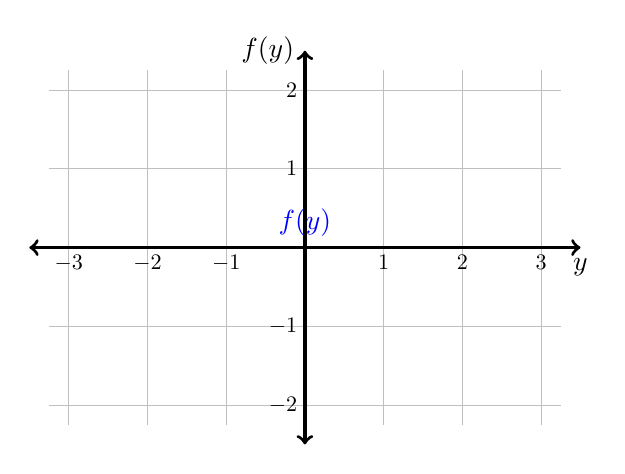
\begin{tikzpicture}
\draw[gray!50] (-3.25,-2.25) grid (3.25,2.25);
\draw[very thick,<->] (-3.5,0) -- (3.5,0) node[below] {$y$};
\draw[very thick,<->] (0,-2.5) -- (0,2.5) node[left] {$f(y)$};
\draw[very thick,color=blue] plot[domain=-3.2:3.2,samples=400] function {10*(x-1)*(x+2)*(x+3)/exp(x/1.4+4)} node[above] {$f(y)$};
\draw (-1,0) node[below, scale=0.8] {$-1$};
\draw (-2,0) node[below, scale=0.8] {$-2$};
\draw (-3,0) node[below, scale=0.8] {$-3$};
\draw (1,0) node[below, scale=0.8] {$1$};
\draw (2,0) node[below, scale=0.8] {$2$};
\draw (3,0) node[below, scale=0.8] {$3$};
\draw (0,2) node[left, scale=0.8] {$2$};
\draw (0,1) node[left, scale=0.8] {$1$};
\draw (0,-1) node[left, scale=0.8] {$-1$};
\draw (0,-2) node[left, scale=0.8] {$-2$};
\end{tikzpicture}
\end{flushright} 
\setcounter{enumCount}{\theenumi}
\end{enumerate}






\end{document}
